\documentclass[12pt,twoside,openright,british]{scrreprt}

\usepackage{microtype}
\usepackage[T1]{fontenc}
\usepackage{lmodern}

% LYX PART
\usepackage{fontspec}
\setmainfont[Ligatures=TeX]{Swis721 Cn BT}
\setsansfont[Ligatures=TeX]{Swis721 Cn BT}
\setmonofont{Swis721 Cn BT}
\usepackage[paperwidth=17cm,paperheight=24cm]{geometry}
\geometry{verbose,tmargin=2cm,bmargin=2.5cm,lmargin=2cm,rmargin=1.2cm}
\setcounter{secnumdepth}{3}
\setcounter{tocdepth}{2} % profondità della Table of Contents
\usepackage[italian, english]{babel}
\usepackage{setspace}
\usepackage[authoryear]{natbib} 
\onehalfspacing
\usepackage[unicode=true,
 bookmarks=true,bookmarksnumbered=false,bookmarksopen=false,
 breaklinks=false,pdfborder={0 0 1},backref=false,colorlinks=false]
 {hyperref}
\hypersetup{pdftitle={PhD thesis Roberto Gentile},
 pdfauthor={Roberto Gentile},
 pdfsubject={Simple Lateral Mechanism Analysis, SLaMA}}

\makeatletter
\@ifundefined{date}{}{\date{}}
\makeatother
% END OF LYX PART


%%% ROB's PART
\usepackage[utf8]{inputenc} 			% codifica che supporta le lettere accentate
\bibliographystyle{agsm} 				% HARVARD BIBLIOGRAPHY
\usepackage{booktabs} 				% per tabelle
\usepackage{multirow}				% celle unite nelle tabelle
\usepackage{paracol} 				% pagine con doppia colonna
\usepackage{float}					% per i float
\usepackage{placeins} 				% per i float
\usepackage{appendix}
\usepackage{amsmath}				% breaks equations in multiple lines
\globalcounter{equation} 				% evitare doppia numerazione delle equazioni per colpa di paracol
\usepackage{array}
\usepackage{lscape} 				% pagina in orizzontale
\usepackage{graphicx}				% scalare le tabelle
\usepackage{rotating} 				% ruotare figure
\usepackage{wrapfig} 				% ruotare le figure
\usepackage{afterpage} 				% mettere figure solo nella pagina sinistra/destra
\usepackage{threeparttable} 			% footnotes sotto le tabelle 
\usepackage[font=footnotesize]{caption} 	% fontSize for captions (if normal is 12, footnotesize is 10)
\usepackage{pdfpages}				% insert external pdfs (e.g. the cover page)

\usepackage{fancyhdr}				% headers with Chapter name etc
\renewcommand*\chapterpagestyle{empty}

\usepackage{titlesec}	% sections and subsections (if normal is 12, large is 14.4 pt: è il più vicino ai 14pt)richiesti)
\titleformat*{\section}{\large\bfseries}
\titleformat*{\subsection}{\bfseries}
\titleformat*{\subsubsection}{\itshape} %per fare come dicono le norme redazionali impostare \large\bfseries per tutti e tre i livelli

\usepackage{hyperref}	% links in the document & table of content in the PDF
\hypersetup{
    bookmarksdepth=4	% bookmarks bar up to the fourth level
    unicode=false,          	% non-Latin characters in Acrobat?s bookmarks
    pdftoolbar=true,        	% show Acrobat?s toolbar?
    pdfmenubar=true,        	% show Acrobat?s menu?
    pdffitwindow=false,     	% window fit to page when opened
    pdfstartview={FitH},    	% fits the width of the page to the window
    pdftitle={My title},    	% title
    pdfauthor={Roberto Gentile},     		% author
    pdfsubject={Simple Lateral Mechanism Analysis, SLaMA},   	% subject of the document
    pdfcreator={Roberto Gentile},   		% creator of the document
    pdfproducer={Roberto Gentile}, 		% producer of the document
    pdfkeywords={keyword1, key2, key3}, 	% list of keywords
    pdfnewwindow=true,   	% links in new PDF window
    colorlinks=false,       	% false: boxed links; true: colored links
    linkcolor=red,          	% color of internal links (change box color with linkbordercolor)
    citecolor=green,        	% color of links to bibliography
    filecolor=magenta,      	% color of file links
    urlcolor=cyan           	% color of external links
}

\DeclareOldFontCommand{\bf}{\normalfont\bfseries}{\mathbf}
%%% END OF ROB's PART



%%% DOCUMENT
\begin{document}


% COVER PAGE
%headers settings
\pagestyle{empty}
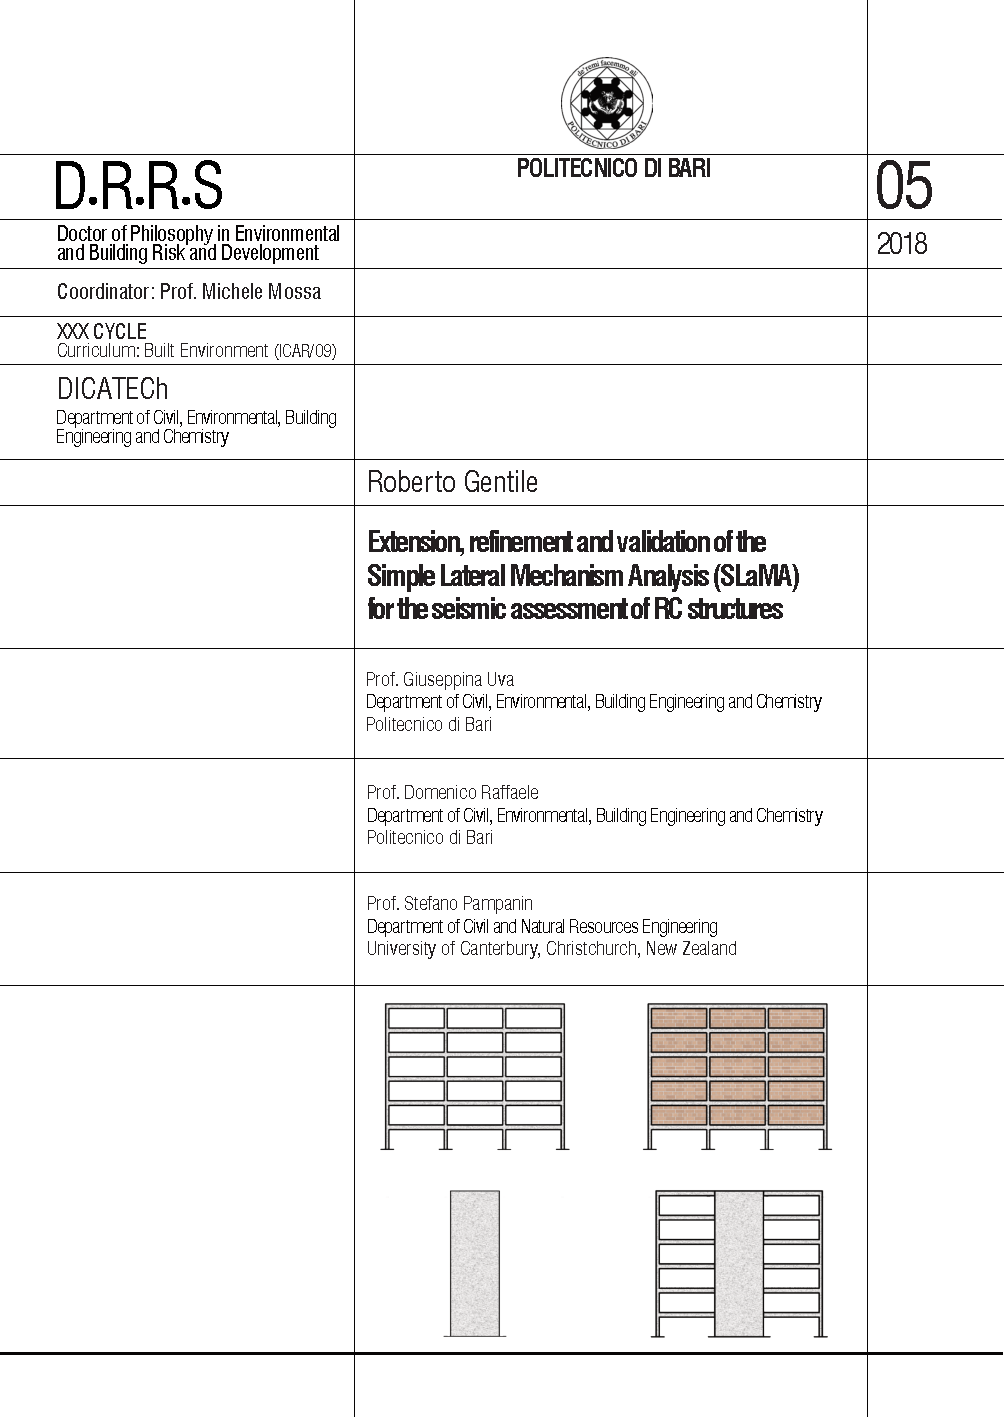
\includepdf[pages={1}, pagecommand={}]{COVERpage/copertinaENG.pdf}
\cleardoublepage
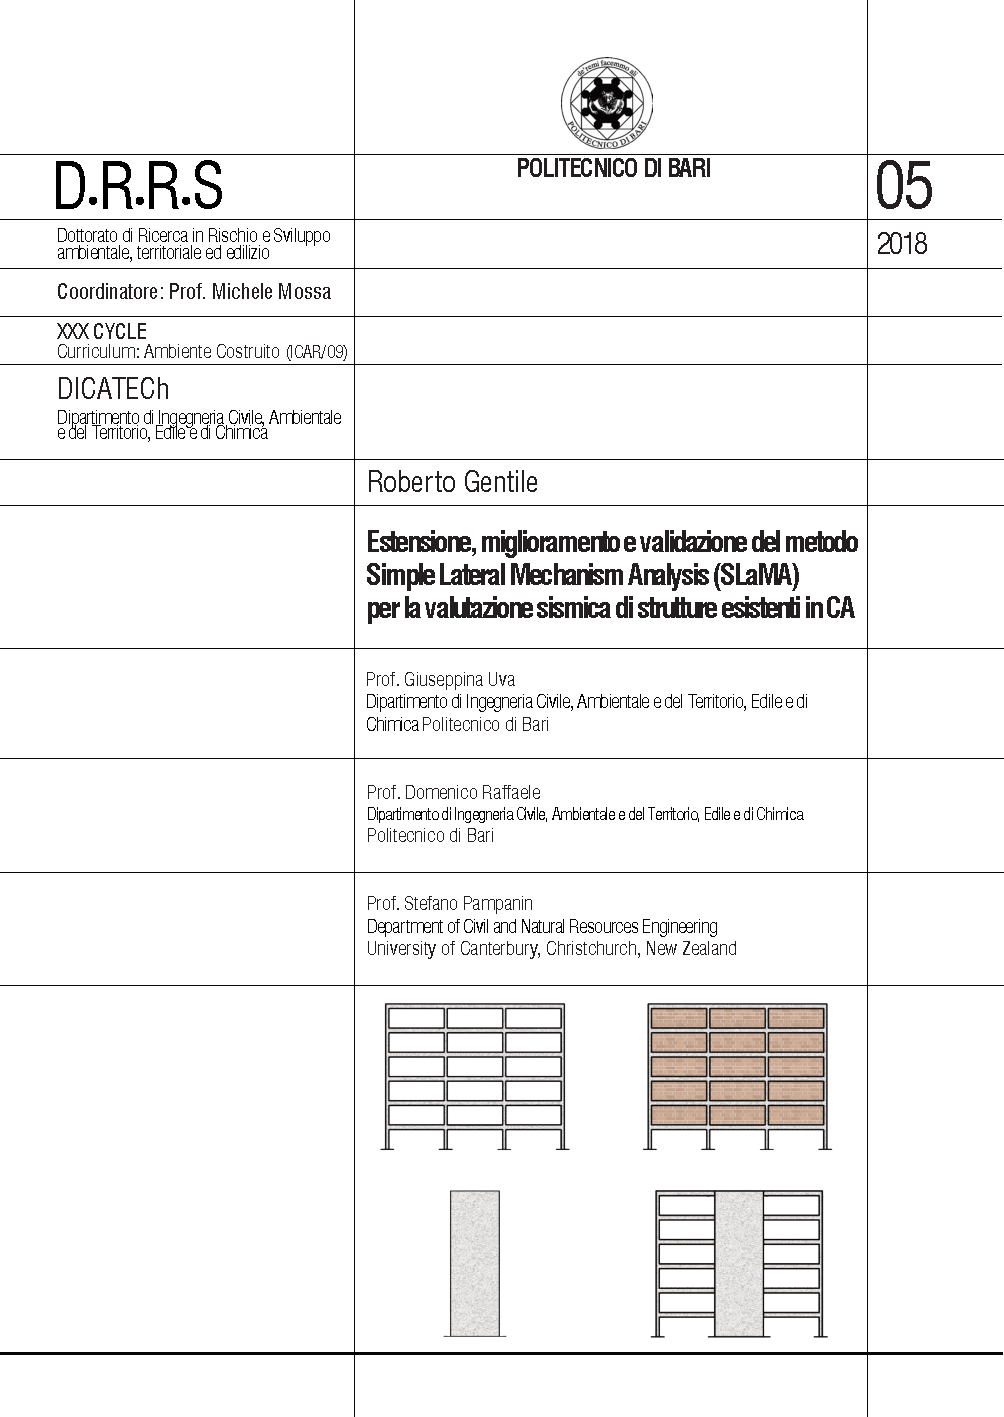
\includepdf[pages={1}, pagecommand={}]{COVERpage/copertinaITA.pdf}


% ABSTRACT
\begin{abstract}

\noindent \textbf{\large Abstract}

This dissertation is focused on the extension, refinement and validation of the Simple Lateral Mechanism Analysis (SLaMA) method for the seismic assessment of RC buildings. Suggested in the 2017 New Zealand guidelines for seismic assessment, \cite{NZSEE2016}, SLaMA is an analytical non-linear analysis technique that provides a first estimation of the global capacity curve of the primary lateral-resisting systems in RC buildings, including bare frames, cantilever walls and dual wall/frame systems. The basic idea is to progress ``from local to global",  extending the local behaviour of the structural members to selected sub-schemes, and finally to the global non-linear response of the building. Inelastic torsional effects are also included. Since simplified assumptions are made, no numerical computer model is needed and hence all the calculations can be performed ``by hand" (i.e. implemented in an electronic spreadsheet). \\

The first part of this investigation is related to bare frame Lateral Resisting Systems, with the identification of  potential areas of improvement for the existing SLaMA procedure and the proposal of an extended/refined one. The refined procedure for bare frames is validated through the application to a set of 40 ideal case studies and the comparison with refined numerical analyses (FEM Pushover). The results show that the refined SLaMA procedure allows to accurately identify the expected plastic mechanism of the frame, also considering the actual hierarchy of strength of its members, and to properly estimate its non-linear capacity curve with acceptable errors on the most meaningful parameters. \\

The subsequent part of the investigation involves the development of a novel SLaMA method to evaluate the capacity curve of masonry-infilled frames systems, which represent a large portion of the building portfolio, especially in Europe. The incorporation of the contribution of the infills is completely absent in the \cite{NZSEE2016} SLaMA framework. The methodology is based on a proposed mechanically-based procedure to decouple the frame and infills contributions to the overturning moment (and hence base shear) capacity for any value of the global displacement. The decoupling procedure is applicable regardless of the distribution of the infills and of the non-linear Axial load-Axial strain of the equivalent struts. It can be applied to post-process the results of Pushover or Time History analyses of different types of infilled frames (material-wise). Similarly to what done for bare frames, an extensive SLaMA vs numerical Pushover comparison, for a set of 72 ideal case studies, is used to validate the proposed SLaMA procedure. \\

Part of the investigation is dedicated to dual wall/frame system structures, proposing a novel SLaMA procedure in which the coupled behaviour of the frame and wall(s) components is expressly considered, including the calculation of the exchanged forces and the concentrated moment couples due to the possible presence of link beams. By using the new SLaMA procedure it is possible to capture the non-linear behaviour of the dual system with extreme accuracy, as demonstrated with an extensive SLaMA vs numerical Pushover parametric analysis comprising 24 ideal case studies. \\

The last step of the work is the seismic assessment of a real case study building, severely damage in the Christchurch (New Zealand) sequence of earthquakes in 2010-2011. Different analysis techniques are used to independently derive the ``seismic score" of the building (capacity over demand), including: Linear Static, Linear Dynamic, Non-Linear Static (numerical Pushover and SLaMA) and Non-Linear Dynamic analyses. Firstly, this demonstrates the reliability of the SLaMA method in assessing real, complex cases by means of a cross-validation. Moreover, and perhaps more importantly, it is deemed that this comparative study demonstrates how the insights gained by using SLaMA can be used to calibrate important parameters needed when adopting other analysis techniques, or interpreting their results. \\

Additional investigations might help in fine-tuning some of its steps but, overall, it is deemed that SLaMA constitutes a robust analysis technique that allows the assessor to really understand the behaviour of an RC building only using hand calculations, possibly implemented in a simple spreadsheet. 

\end{abstract}


\begin{abstract}

%\begin{otherlanguage}{italian}

\textbf{\large Sommario}

Il lavoro in questa tesi riguarda l'estensione, il miglioramento e la validazione della metodologia Simple Lateral Mechanism Analysis (SLaMA) per la valutazione sismica di strutture in CA. Raccomandato nelle linee guida neozelandesi del 2017 relative alla valutazione sismica, \cite{NZSEE2016}, SLaMA \'e un metodo di analisi non-lineare che permette di avere una stima della capacit\'a di strutture esistenti ed \'e valido per telai, pareti o sistemi misti telaio/parete. L'idea di base \'e procedere ``dal locale al globale", partendo dal comportamento di componenti singoli, estendendolo a specifici sottoschemi ed infine giungendo al comportamento globale dell'edificio. \'E anche possibile considerare gli effetti torsionali in campo non-lineare. Dato che il metodo si basa su ipotesi semplificate, non \'e necessario ricorrere a modelli numerici e i calcoli possono essere fatti ``a mano" (i.e. utilizzando un foglio elettronico). \\

La prima parte di questo lavoro di ricerca riguarda i sistemi a telaio nudo, identificando aree di miglioramento della procedura SLaMA esistente e proponendo una procedura estesa e migliorata. Essa \'e stata validata attraverso la sua applicazione a 40 casi studio ideali e il confronto con i risultati di analisi numeriche raffinate (FEM Pushover). I risultati indicano che la procedura SLaMA modificata permette di identificare accuratamente il meccanismo plastico del telaio, considerando l'effettiva gerarchia delle resistenze dei suoi componenti, e di calcolarne la curva di capacit\'a con errori accettabili per i suoi parametri più significativi. \\

La parte successiva del lavoro riguarda lo sviluppo di una nuova procedura SLaMA, non presente in \cite{NZSEE2016}, per sistemi a telaio tamponato, che rappresentano una cospicua parte del patrimonio edilizio, soprattutto in Europa. La nuova metodologia si basa su una procedura meccanica, proposta in questo lavoro, per disaccoppiare i contributi al taglio alla base relativi al telaio e alle tamponature, per un qualunque valore dello spostamento globale. La procedura di disaggregazione \'e applicabile a prescindere dalla distribuzione delle tamponature e della curva caratteristica dei puntoni equivalenti. Pu\'o essere inoltre applicata per la post-processione dei risultati di analisi Pushover o Time History di telai tamponati. In analogia a quanto fatto per i telai nudi la procedura SLaMA \'e stata validata tramite confronto con i risultati di analisi Pushover per 72 casi studio. \\

Sono stati inoltre considerati i sistemi resistenti misti telaio/parete con l'obiettivo di proporre una nuova procedura SLaMA che considerasse esplicitamente l'interazione tra la parte a telaio con quella a parete, includendo il calcolo delle forze da essi scambiate e le eventuali coppie concentrate dovute alla presenza di travi di collegamento. Con la nuova procedura SLaMA \'e possibile stimare il comportamento dei sistemi duali con grande accuratezza, come dimostrato da una vasta analisi parametrica (SLaMA vs Pushover) che coinvolge 24 casi studio. \\

L'ultima parte del lavoro riguarda la valutazione sismica di un edificio realmente esistito e che ha subito notevoli danni durante la sequenza sismica di Christchurch (Nuova Zelanda) tra il 2010 e il 2011. Lo ``score sismico" (capacit\'a fratto domanda) \'e stato indipendentemente valutato con diversi metodi di analisi: Lineare Statica, Lineare Dinamica, Non-Lineare Statica (Pushover e SLaMA), Non-Lineare Dinamica. In primis questo confronto incrociato dimostra l'affidabilit\'a del metodo SLaMA nella valutazione di casi reali complessi. Questo studio dimostra inoltre come le informazioni ottenute utilizzando SLaMA possano essere efficacemente usate per calibrare i parametri fondamentali necessari per gli altri metodi di analisi, o interpretarne i risultati. \\

Sebbene alcuni passi della procedura possono essere calibrati in maniera pi\'u raffinata grazie a sviluppi futuri si pu\'o sicuramente affermare che SLaMA sia un metodo di analisi robusto. Esso \'e in grado di fornire al tecnico valutatore gli strumenti per comprendere i dettagli del comportamento di un edificio usando esclusivamente calcoli fatti a mano (eventualmente implementati in un semplice foglio elettronico).

%\end{otherlanguage}

\end{abstract}

%\TableOfContents OLD
\tableofcontents\label{toc}

\pagestyle{fancy}
\fancyhf{}
\fancyhead[RO]{Roberto Gentile}
\fancyhead[LE]{\scriptsize \leftmark}
\fancyfoot[LE,RO]{\thepage}
%\fancyfoot[RE,LO]{\hyperref[toc]{\footnotesize Go to ToC}}


%\NonNumChapter{\textit{Introduction}} OLD
\chapter*{\textit{Introduction}}
\label{chap:intro}
\addcontentsline{toc}{chapter}{Introduction}
\section*{Background} 
\addcontentsline{toc}{section}{Background}

Seismic assessment of existing structures is a complex procedure characterised by the definition of the expected seismic demand (hazard) and structural capacity (vulnerability). Generally, the \textit{seismic score} of the analysed structure is obtained by comparing demand and capacity. It is commonly accepted that seismic assessment is not a prediction of the actual performance of a structure under a particular seismic attack but instead is the general understanding of the likely behaviour of the structure under a certain level of the seismic demand.


\section*{Research motivations}
\addcontentsline{toc}{section}{Research motivations}

The SLaMA method originates from pioneering literature works regarding RC frames and cantilever wall structures , \cite{priestley1991}, \cite{park1995}, \cite{priestley1997}. The method was firstly introduced in the 2006 New Zealand seismic assessment guidelines. \cite{NZSEE2006}. In \cite{kam2013}, some practical considerations are drawn regarding to its application in seismic assessment of real buildings. Finally, a revamped version of SLaMA was introduced in the 2017 New Zealand guidelines on seismic assessment, \cite{NZSEE2016}, in which a tentative procedure for dual wall/frame systems was also introduced.


\section*{Hypothesis, objectives and scope}
\addcontentsline{toc}{section}{Hypothesis, objectives and scope}


This research work seeks to demonstrate the subsequent hypothesis: \\

\textit{SLaMA is a simple yet reliable method to obtain a first estimation of the capacity curve and the expected plastic mechanisms of an RC building with a Lateral Resisting System composed of frames (bare or masonry-infilled), cantilever walls and/or dual wall/frame systems.}\\


\section*{Research methodology and division of the work}
\addcontentsline{toc}{section}{Research methodology and division of the work}

To meet the objectives of this study, the work was divided into 4 phases, as shown in the Figure here below. 

Specific tasks were individuated for this work, one for each phase, and they are listed here below:



\section*{Dissertation outline}
\addcontentsline{toc}{section}{Dissertation outline}

Apart from this general \textbf{Introduction}, the dissertation is outlined as follows.\\

\textbf{Chapter \ref{chap:assessment}} gives a general overview and critical comparison of the code-based approaches for seismic vulnerability assessment of existing buildings, as suggested in the most important international standards. The conceptual approaches of three selected standards (EuroCode 8 - part 3, ASCE 41-13, NZSEE 2017) are compared. The mostly adopted analysis techniques are discussed, focusing on the different assumptions made in the selected standards/guidelines. \\

The \textbf{Conclusions} drawn from this PhD thesis work are finally listed, also recommending future developments.





%\StartOfNumChapters

% CHAPTER 1
\setchapterpreamble{%
    
    \vspace{24pt}
    
    \textbf{{\Large Abstract}}
        
The assessment of the seismic performance of existing buildings is a complex process since, typically, those are not specifically designed to resist earthquakes. With respect to new structures, more advanced and detailed modelling, analysis and verification procedures are needed, since existing buildings are not specifically designed to exclude a priori the formation of unfavourable, local and global failure mechanisms, which may be difficult to analyse. In this Chapter, the assessment standards/guidelines applied in USA (ASCE 41-13), Europe (EuroCode 8, part 3) and New Zealand (NZSEE 2017) at the time of this thesis work are discussed and compared both in terms of basic principles and suggested analysis techniques.
    
    \vspace{24pt}
    
    \textbf{{\Large Contents}}
    
    \begin{itemize}
    	\item Seismic assessment of existing buildings;
    	\item Comparison of code-based approaches;
    	\item EuroCode 8, part 3, ASCE 41-13, NZSEE 2017.
    \end{itemize}
}

%\NumChapter{\textit{Seismic assessment of existing buildings: code-based approaches}}
\chapter{\textit{Seismic assessment of existing buildings: code-based approaches}}
\label{chap:assessment}
\section{Introduction}

% MARKER: ho detto che i materiali vanno caratterizzati con la resistenza media?
% MARKER: guidelines/standards invece che altra roba

% MARKER: citare che NZSEE permette di usare ASCE 41 o EC8 a patto di calcolare NBS

The assessment of the seismic performance of existing buildings is a complex process since, typically, those are not specifically designed to resist earthquakes. With respect to new structures, more advanced and detailed modelling, analysis and verification procedures are needed, since existing buildings are not specifically designed to exclude a priori the formation of unfavourable, local and global failure mechanisms, which may be difficult to analyse.

The understanding of the structural behaviour of structures under seismic attack has significantly evolved in the last decades, starting in the 1970s with the concept of capacity design, introduced in New Zealand, \cite{hollings1969}, and finally developed in a pioneering book by \cite{park1975}. Considering the high expansion of the cities in the second half of the XX century, it can be stated that a considerable number of the existing buildings was designed having little or no consideration of the seismic actions.

Also the realisation of the existence of a large portfolio of structures subjected to high seismic risk evolved with time, with a step-change in the 1980s, after several human lives and economic losses caused by major earthquakes around the world (e.g. 1989 Loma Prieta, USA, 1995 Kobe, Japan, 1999 Izmit, Turkey, among others).

Clearly, great research effort was sustained in earthquake-risk areas in the world (USA, New Zealand, Japan, Europe) aiming to give recommendations and/or provisions for the assessment of existing structures. For this reason, the best seismic assessment standards/guidelines are written in these regions.

In this Chapter, the assessment standards/guidelines applied in USA, Europe and New Zealand at the time of this thesis work are discussed and compared both in terms of basic principles and suggested analysis techniques. It is worth noting that the European standards are almost entirely implemented in the Italian standards, with minor modifications. The Japanese standards are not included, considering the difficulty in finding up-to-date documents in english language.

Finally, a critical comparison of the considered guidelines/standards is drawn to highlight both good practices and improvable aspects of the selected approaches.


\section{Basic principles of the considered codes}

The guidelines/standards for seismic assessment in USA, Europe and New Zealand are compared in terms of general principles, considered limit states, allowed analysis methods, safety verifications and suggested models for the calculation of the capacity of the members. The analysis methods are described in more detail in Section \ref{codes:methods}.


\subsection{ASCE 41- 13}

The USA standards document \cite{ASCE41}, \textit{Seismic Evaluation and Retrofit of Existing Buildings} (Figure \ref{fig:ASCEcover}) is the result of the update and combination of \cite{ASCE31} related to seismic assessment procedures and \cite{ASCE41-06} related to retrofit interventions. This document is comprehensive of all technical advances in the field collected in the recent years up to 2013.

\begin{figure}[h]
\begin{center}
    
\includegraphics[width=1\textwidth]{./CHAP1/img/ASCEcover}
\caption{Seismic Evaluation and Retrofit of Existing Buildings (cover), modified after \cite{ASCE41}.}
\label{fig:ASCEcover}
\end{center}
\end{figure}


\begin{table}[!h] %MARKER: posizione tabella
\footnotesize
\centering
\caption{Criteria to qualify for the different knowledge levels.}
\label{tab:EC8criteria}
\begin{tabular}{cccccc}
\toprule
\begin{tabular}[c]{@{}l@{}}Knowledge\\ Level\end{tabular} & Geometry                                                                                                                                          & Details                                                                                                                                                                          & Materials                                                                                                                                                  & CF                                                     \\ \midrule
KL1                                                       & \begin{tabular}[c]{@{}l@{}}From original\\ outline\\ construction\\ drawings with\\ sample visual\\ survey\\ or\\ from full\\ survey\end{tabular} & \begin{tabular}[c]{@{}l@{}}Simulated design in\\ accordance with\\ relevant practice\\ and,from limited in-situ\\ inspection\end{tabular}                                        & \begin{tabular}[c]{@{}l@{}}Default values in\\ accordance with\\ standards of the\\ time of construction\\ and from limited\\ in-situ testing\end{tabular} & \begin{tabular}[c]{@{}l@{}}$CF_{KL1}$\\ (1.35)\end{tabular} \\
KL2                                                       & as for KL1                                                                                                                                        & \begin{tabular}[c]{@{}l@{}}From incomplete\\ original detailed\\ construction drawings\\ with limited in-situ\\ inspection\\ or from extended in-\\ situ inspection\end{tabular} & \begin{tabular}[c]{@{}l@{}}From original\\ design\\ specifications with\\ limited in-situ\\ testing\\ or from extended\\ in-situ testing\end{tabular}      & \begin{tabular}[c]{@{}l@{}}$CF_{KL2}$\\ (1.2)\end{tabular}  \\
KL3                                                       & as for KL1                                                                                                                                        & \begin{tabular}[c]{@{}l@{}}From original detailed\\ construction drawings\\ with limited in-situ\\ inspection\\ or from\\ comprehensive in-situ\\ inspection\end{tabular}        & \begin{tabular}[c]{@{}l@{}}From original test\\ reports with limited\\ in-situ testing\\ or from\\ comprehensive in-\\ situ testing\end{tabular}           & \begin{tabular}[c]{@{}l@{}}$CF_{KL3}$\\ (1.0)\end{tabular}  \\ \bottomrule
\end{tabular}
\end{table}




% CHAPTER 1


% CONCLUSIONS
%\NonNumChapter{\textit{Conclusions and future developments}}
\chapter*{\textit{Conclusions and future developments}}
\label{chap:conclusions}
\addcontentsline{toc}{chapter}{Conclusions and future developments}
\section*{Summary}
\addcontentsline{toc}{section}{Summary}



\section*{Key findings and contributions}
\addcontentsline{toc}{section}{Key findings and contributions}


\section*{Overall conclusion}
\addcontentsline{toc}{section}{Overall conclusion}




%% NOTES
%\NonNumChapter{Note}


% REFERENCES
%\NonNumChapter{\textit{References}}
   
    %\bibliographystyle{unsrtnat} 				%STILE DELLA BIBLIOGRAFIA (mettere plain o alpha)
    %\setcitestyle{authoryear, open={},close={}}		%STILE DELLE CITAZIONI
        
%insert bibliography
\renewcommand{\bibname}{References}	% name the bibliography section with "References"
\bibliography{references.bib}
\addcontentsline{toc}{chapter}{References} % appear in the table of contents

\begin{appendices} % MARKER: this can be eliminated

\chapter{Hierarchy of strength: step-by-step numerical example}
\label{app:hierarchy}
% MARKER: check positioning of the figures/tables and put float barriers and/or clearpages if needed

\section{Structural details of the subassembly}
\label{hier:details}

\begin{equation}
\label{eq:EBMjoint}
EBM_{v,j} = \frac{V_{jh}}{\frac{1}{jd}-\frac{l_{b}}{l_{c}l_{b}^{'}}} = \frac{365(699.5)}{\frac{1}{0.628}-\frac{3.4}{3.05*3.17}} = 294.2 kNm (563.8kN \ Pull)
\end{equation}


\end{appendices}

%% ATTACHMENTS

\setchapterpreamble{%
    
I would like to thank the eternal genius of prof Ulysses R. Garbaggio.

}

\chapter*{Acknowledgements}
\addcontentsline{toc}{chapter}{Acknowledgements} % appear in the table of contents

\chapter*{Curriculum Vitae}
\addcontentsline{toc}{chapter}{Curriculum Vitae} % appear in the table of contents

\pagestyle{empty}
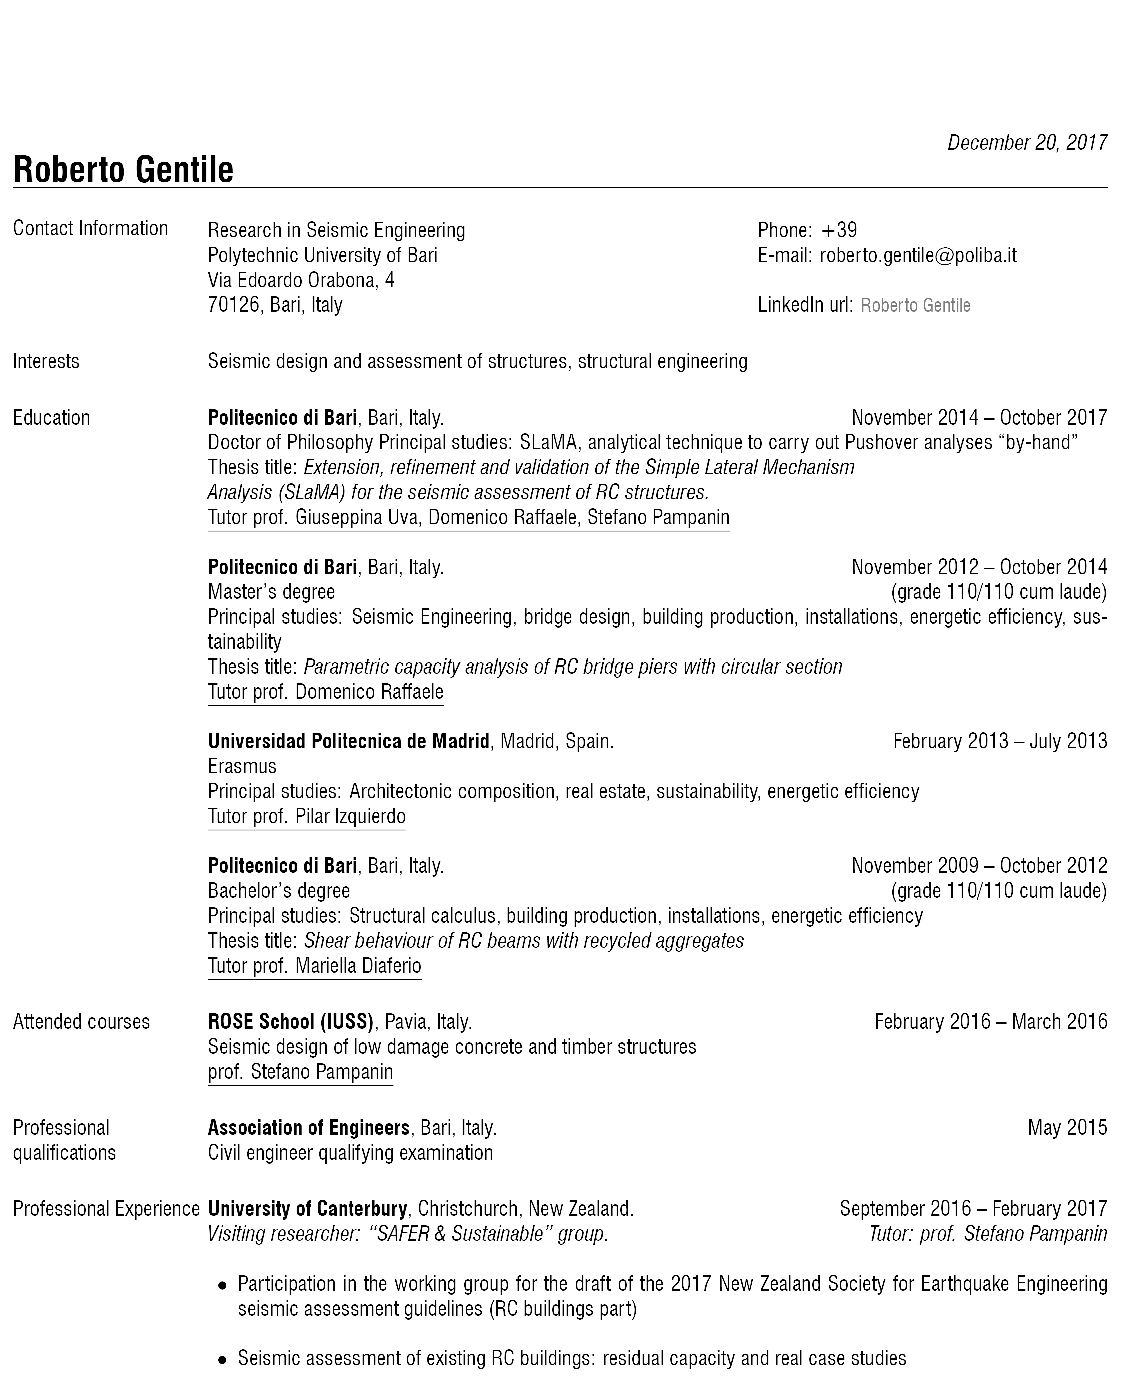
\includepdf[pages={1}, pagecommand={}]{PhDcurriculum.pdf}



\end{document}
